\documentclass[pdfpagelabels=false, usepdftitle=false, aspectratio=169]{beamer}
% \usetheme[navigation, sectiontitles]{UM}
\usetheme[sectiontitles]{UM}
\setcounter{tocdepth}{1}

% ----------------------
% title page information
% ----------------------

\title[Short Title]{Desarrollo de un sistema de programación automatizada de tareas de mantenimiento en la industria minera}
\subtitle{This is a subtitle}

\author[Me, other]{
  Emilio Bravo Maturana
}

\institute[UM]{
  \inst{1} ROA, Maastricht University \\
  \inst{2} SBE, Maastricht University
}

\date{\today}


% ---------------------
% begin of presentation
% ---------------------

\begin{document}


\UMtitleframe  % note that we *do not* use \titlepage


% ----Frame------------

\begin{frame}{Agenda}
    \tableofcontents
\end{frame}


% ----------------------------------------------
% Sección: Resumen Ejecutivo
% ----------------------------------------------

\section{Resumen Ejecutivo}

% --- FRAME 1 ---
\begin{frame}{Programación de Actividades de Mantenimiento}
\begin{itemize}
    \item El mantenimiento eficiente de equipos es crucial para garantizar la continuidad operativa en cualquier industria.
    \vfill
    \item Las \textbf{restricciones de recursos} y las ventanas temporales son factores que complejizan el proceso de programación.
    \vfill
    \item La programación manual de actividades de mantenimiento:
    \begin{itemize}
        \item Es compleja e intensiva en tiempo.
        \item Es propensa a errores debido a múltiples variables.
        \item Depende altamente de personal especializado.
    \end{itemize}
\end{itemize}
\vfill
\end{frame}


% --- FRAME 2 ---
\begin{frame}{Propuesta de Automatización}
\begin{block}{Objetivo Principal}
    Automatizar la programación de tareas de mantenimiento mediante herramientas avanzadas de modelado y optimización.
\end{block}
\vfill
\begin{itemize}
    \item El problema se modela como un Problema de Programación de Proyectos con Restricciones de Recursos (\textit{RCPSP}).
    \vfill
    \item Se utilizan técnicas de Programación por Restricciones (\textit{Constraint Programming, CP}) para encontrar soluciones eficientes.
\end{itemize}
\vfill
\end{frame}

% --- FRAME 2: Ejemplo de Gantt en MS Project ---
\begin{frame}{Programación de Actividades}
    \centering
    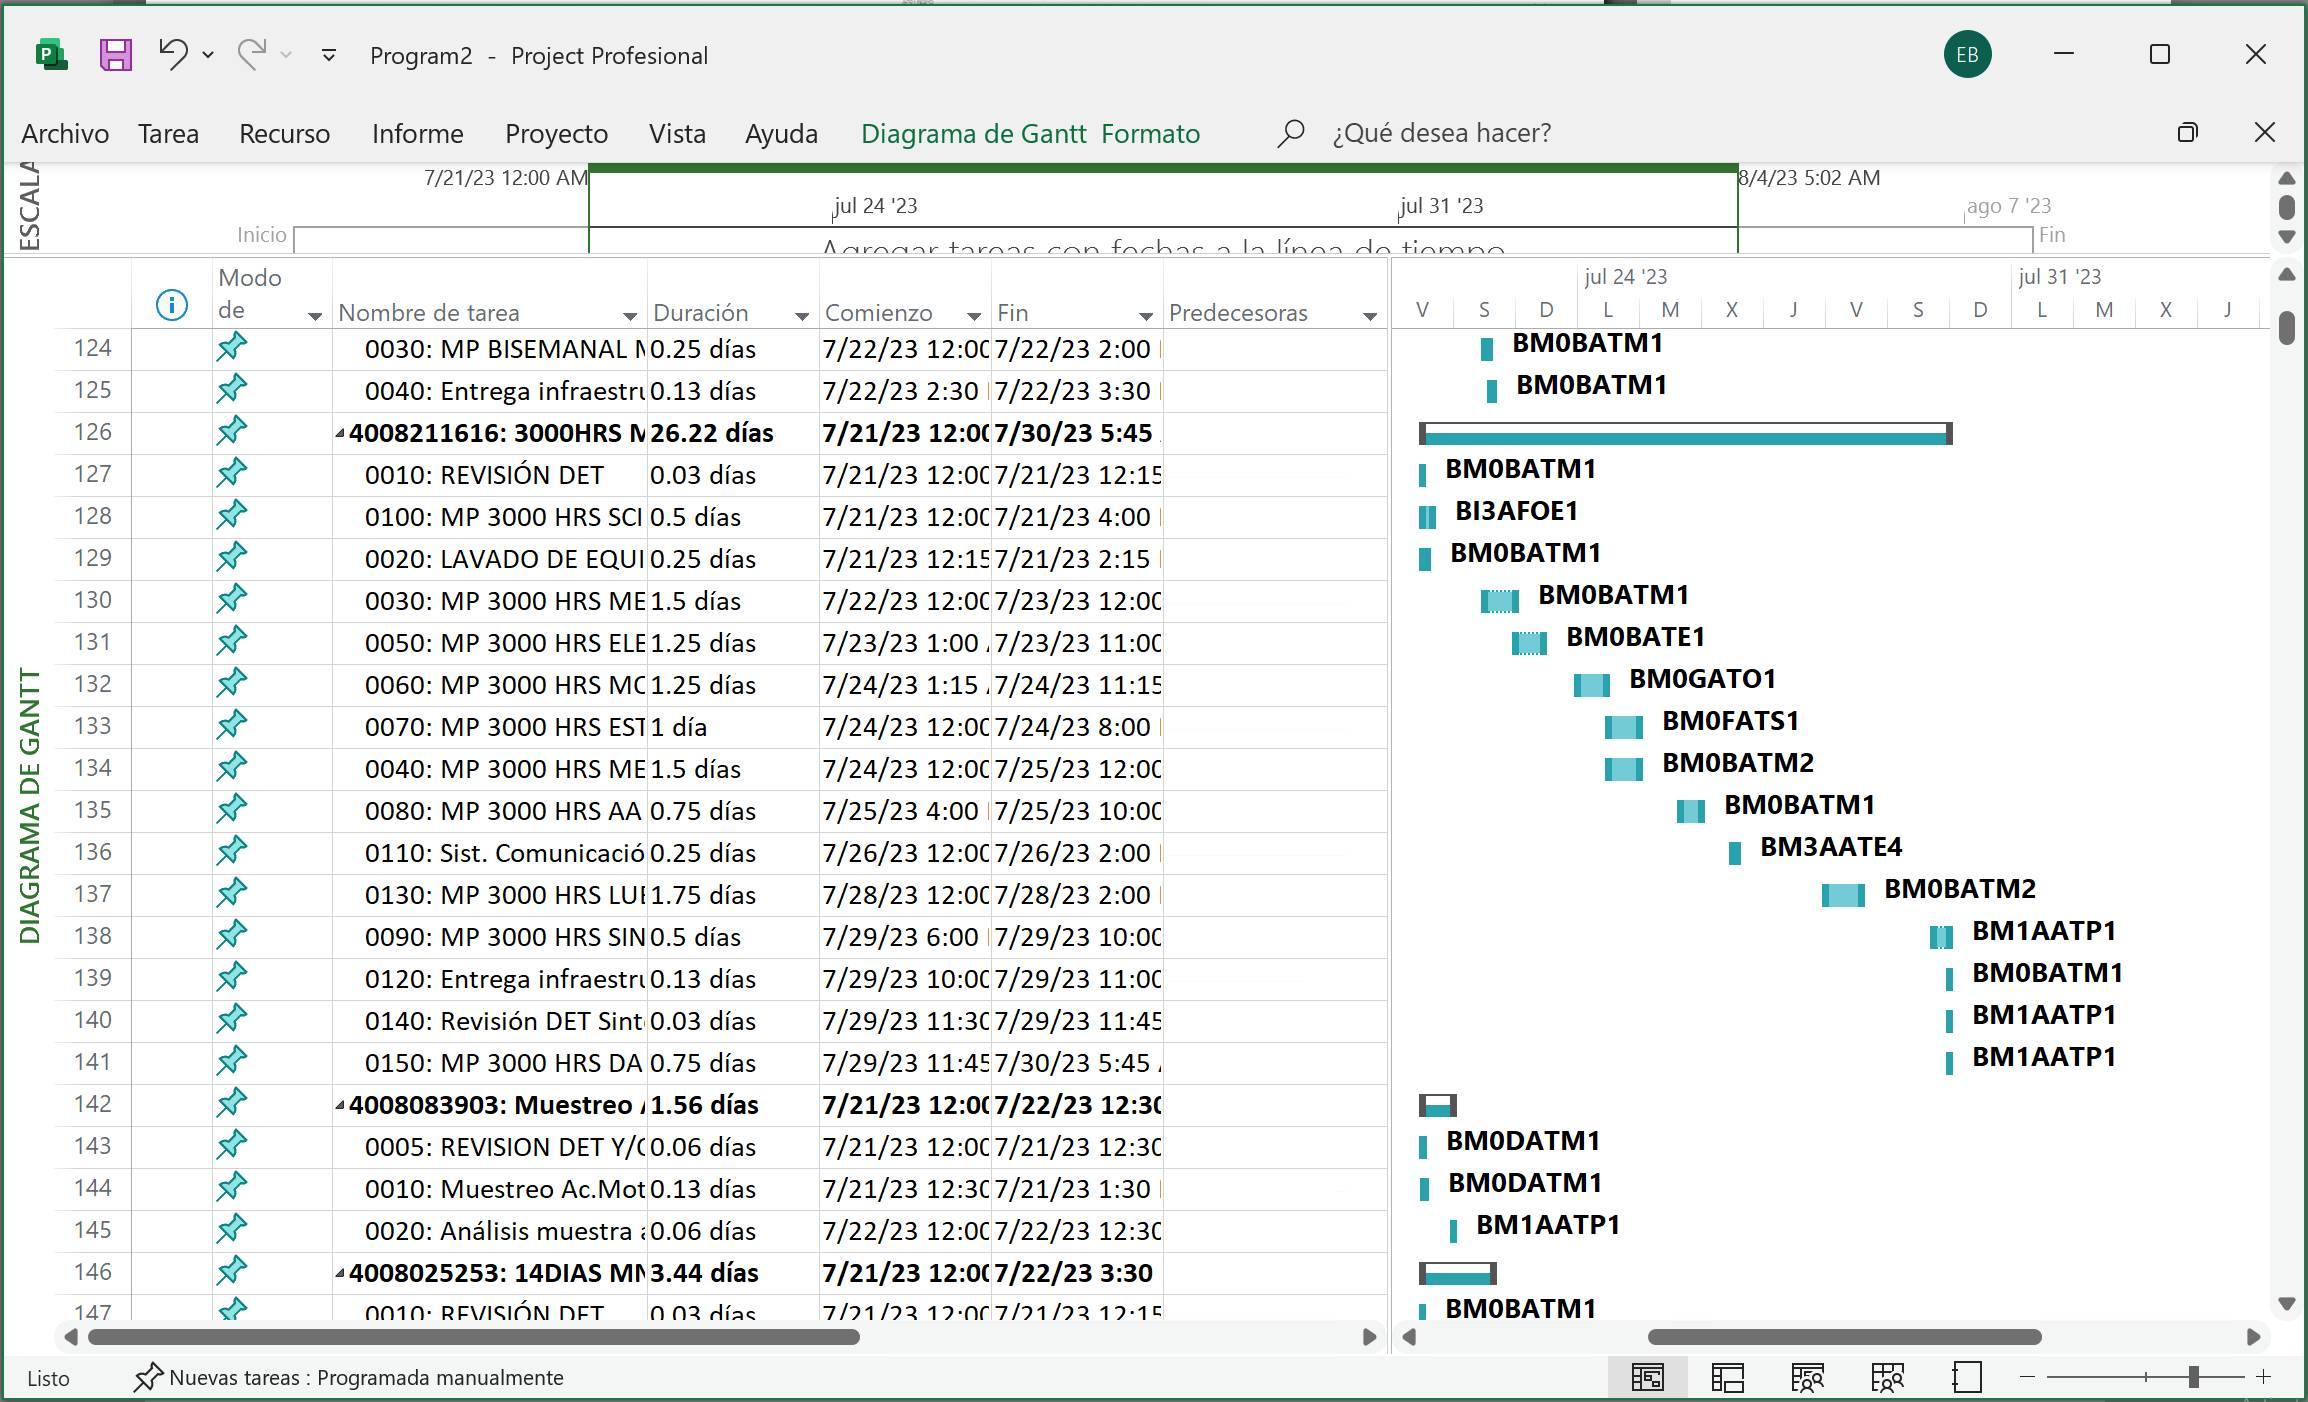
\includegraphics[scale=0.2]{imgs/gantt-project.jpg}
    \captionof{figure}{Captura de Cronograma Resultante en \textit{MS Project} \cite{refMSProject}.}
    \label{fig:gantt-project}
    \vfill
    \end{frame}


\begin{frame}{Impacto de la Solución}
    Un correcto diseño e implementación de la solución propuesta permitirá:
    \vfill
\begin{itemize}
    \item \textbf{Optimización del tiempo y esfuerzo:} Liberación del equipo de programación de tareas manuales intensivas.
    \item \textbf{Reducción de errores:} Especialmente aquellos derivados de programaciones deficientes.
\end{itemize}
\vfill

\end{frame}

\begin{frame}{Resultados Obtenidos}
\begin{itemize}
    \item Cronograma generado para \textbf{4.898 tareas}.
    \item Programación del 98,6\% de las tareas.
    \item \textit{Makespan} (Tiempo total del proyecto): 21,5 días.
    \item Tiempo de procesamiento: \textbf{6,12 segundos}.
\end{itemize}
\vfill
\end{frame}


% ----------------------------------------------
% Sección: Análisis y descripción del problema
% ----------------------------------------------

\section{Análisis y descripción del problema}

% --- FRAME 3: Visión General ---
\begin{frame}{Levantamiento del Proceso de Programación}
\begin{itemize}
    \item \textbf{Objetivo:} Generalizar el proceso de programación de tareas en la empresa colaboradora.
    \vfill
    \item \textbf{Metodología:}
    \begin{itemize}
        \arrowitem Análisis de documentos normativos del proceso.
        \arrowitem Encuesta dirigida al personal encargado de la programación.
    \end{itemize}
    \vfill
    \item Este análisis permitió:
    \begin{itemize}
        \arrowitem Comprender el funcionamiento operativo actual.
        \arrowitem Identificar barreras y desafíos.
        \arrowitem Validar la necesidad de una solución automatizada.
    \end{itemize}
\end{itemize}
\vfill
\end{frame}

% --- FRAME 7: Ciclo Semanal de Programación ---
\begin{frame}{Ciclo Semanal de Programación}
    \begin{figure}
        \centering
        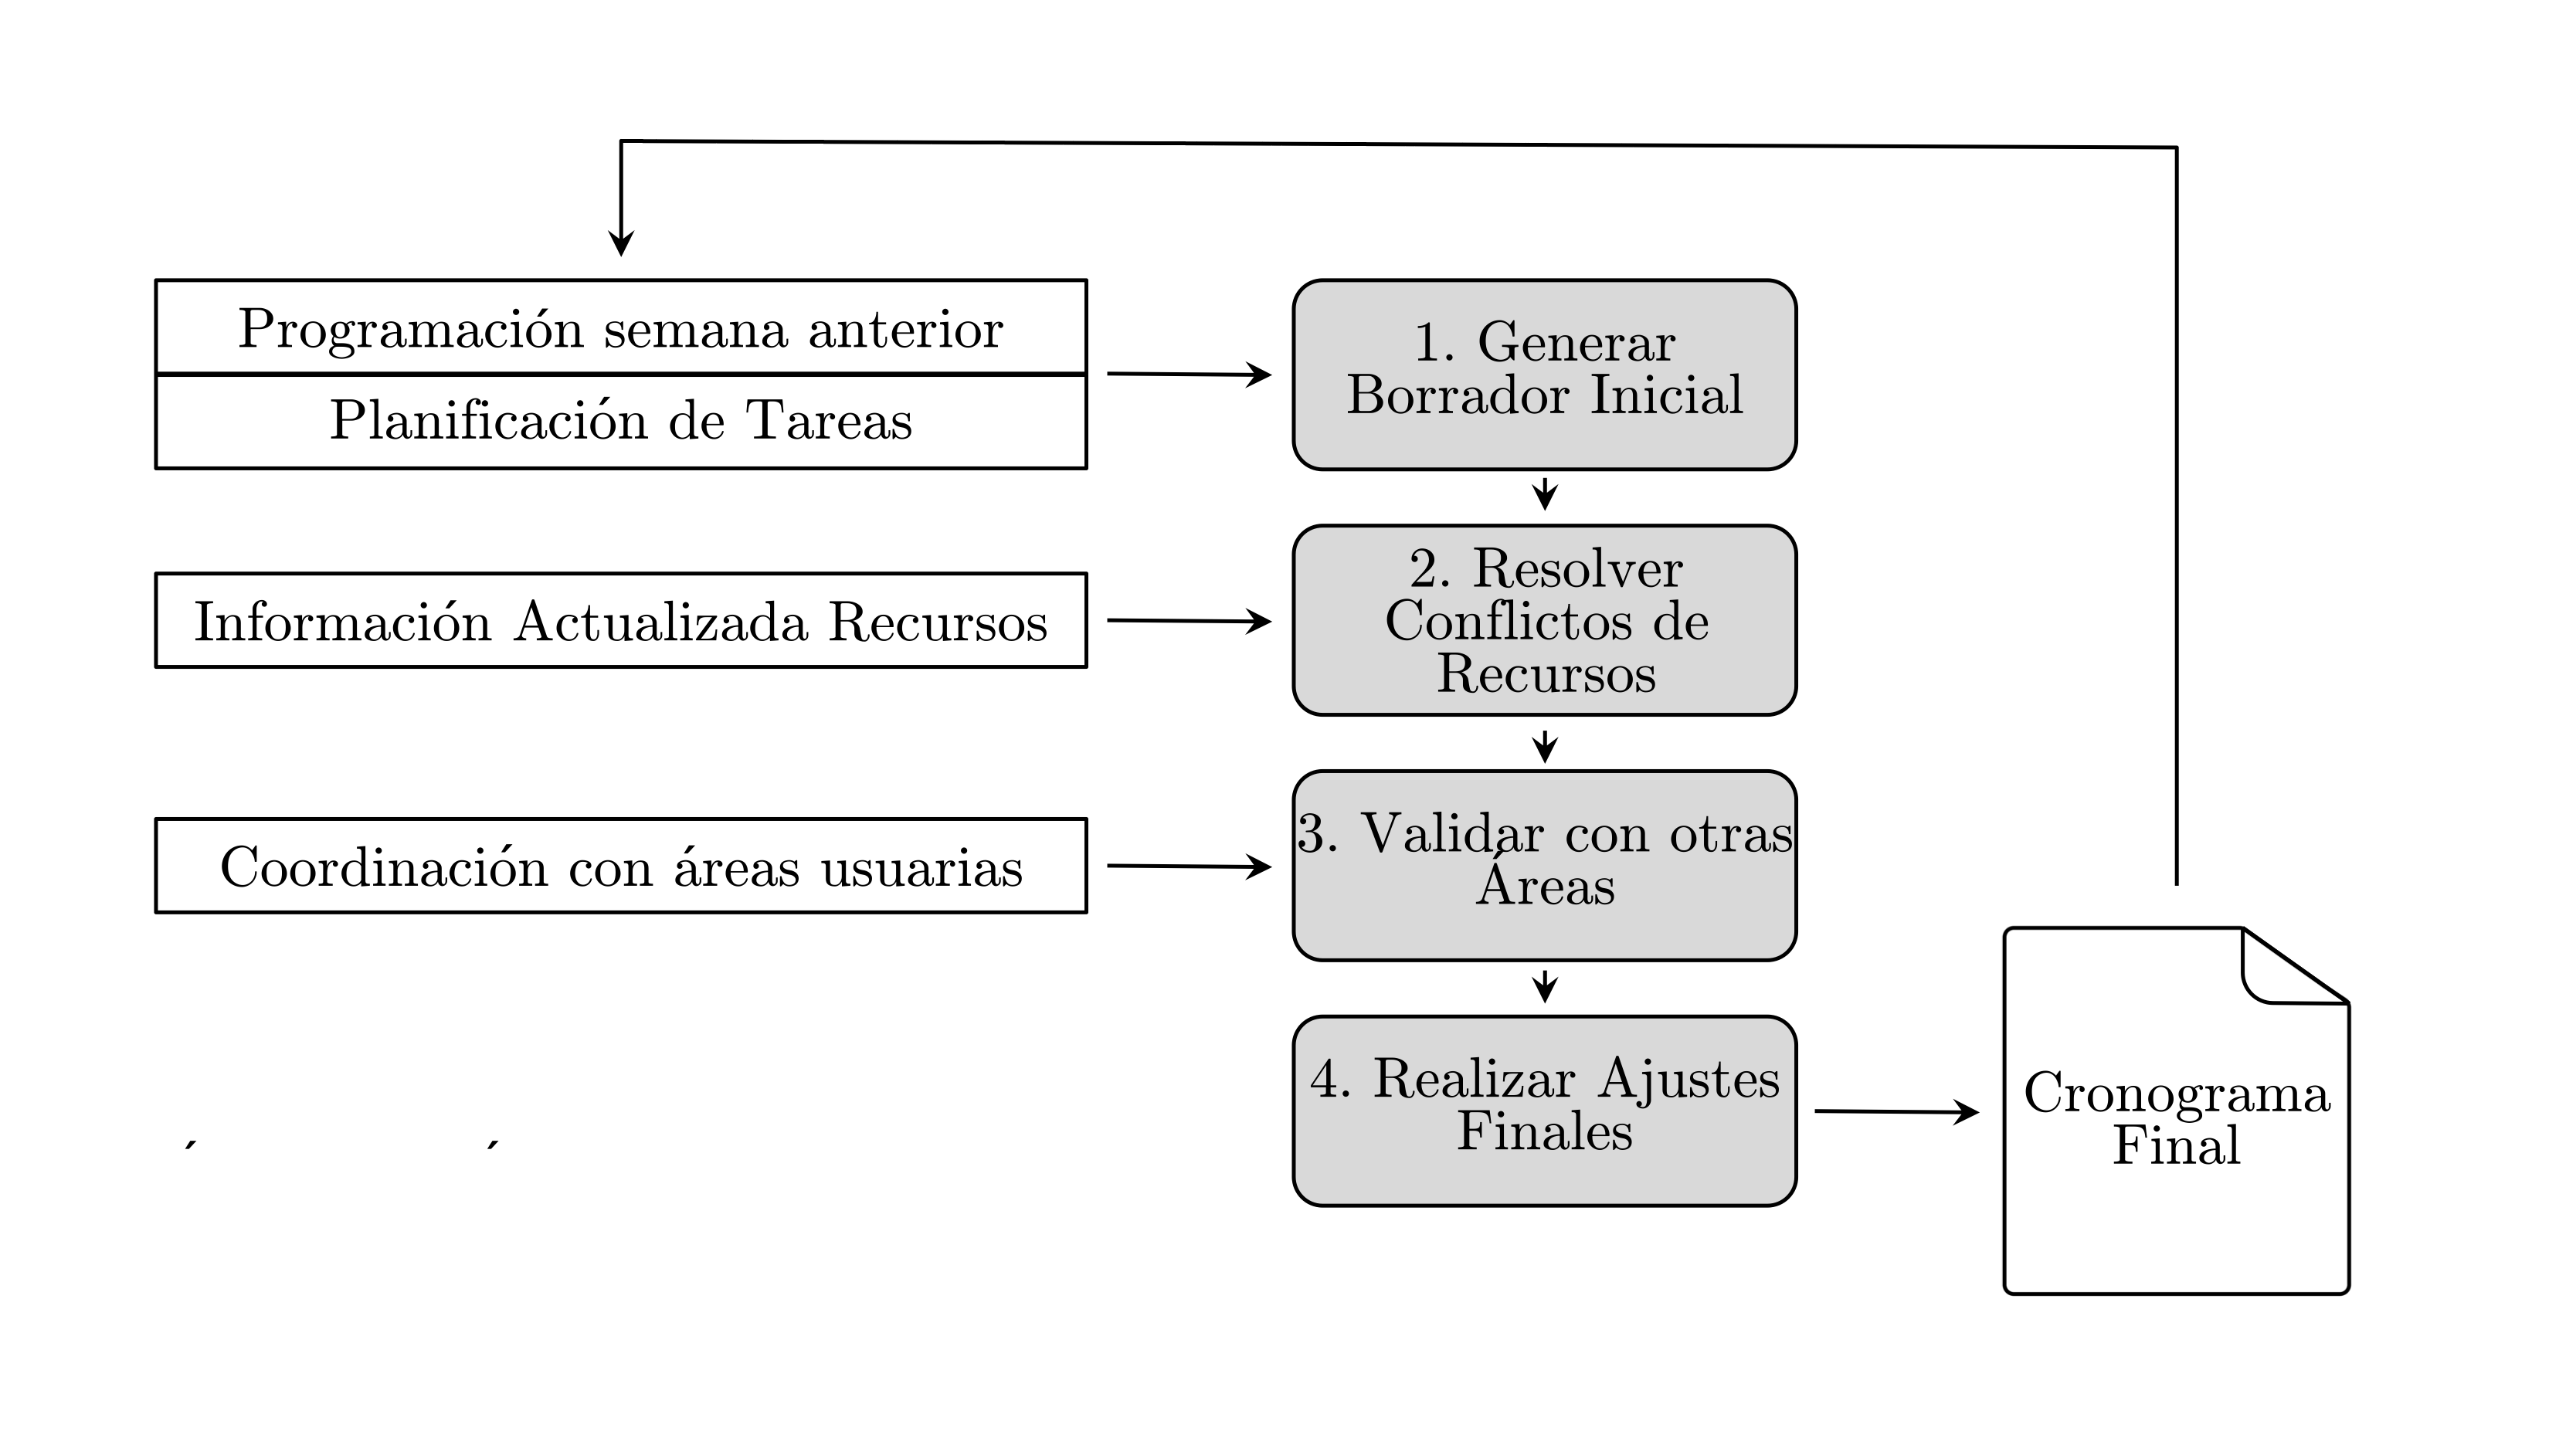
\includegraphics[width=0.66\textwidth]{imgs/process_flowchart.png}
        \caption{Ciclo Semanal de Programación de Actividades.}
        \label{fig:flowchart}
    \end{figure}
    \vfill
    \end{frame}


% --- FRAME 7: Ciclo Semanal de Programación ---
% \begin{frame}{Ciclo Semanal de Programación}
%     \begin{itemize}
%         \item Se revisa y ajusta el cronograma cada semana (miércoles), incorporando nuevas tareas.
%         \item El borrador del cronograma para las próximas tres semanas se valida con otras áreas.
%         \item Cada viernes se emite el cronograma oficial, base del siguiente ciclo iterativo.
%     \end{itemize}
%     \vfill
%     \end{frame}

% --- FRAME 4: Descripción General del Proceso ---
% \subsection{Descripción del proceso de programación}
% \begin{frame}{Descripción General del Proceso}
% \begin{itemize}
%     \item El proceso de programación de tareas se sustenta en la planificación previa, que define las ventanas temporales iniciales.
%     \vfill
%     \item El equipo de programación:
%     \begin{itemize}
%         \arrowitem Ajusta las tareas a las restricciones reales de recursos.
%         \arrowitem Itera semanalmente para mantener el cronograma actualizado.
%     \end{itemize}
%     \vfill
%     \item \textbf{Elementos clave:} Ventanas temporales, disponibilidad de recursos, coordinación con áreas involucradas, criticidad de tareas.
% \end{itemize}
% \vfill
% \end{frame}

% --- FRAME 5: Proceso de Planificación ---
% \subsubsection{Proceso de planificación}
% \begin{frame}{Proceso de Planificación}
% \begin{itemize}
%     \item Responsables de definir ventanas temporales y requerimientos de mantenimiento.
%     \item Consideraciones:
%     \begin{itemize}
%         \arrowitem Objetivos estratégicos de la mina.
%         \arrowitem Tiempos de procesos industriales.
%         \arrowitem Otros factores del negocio minero.
%     \end{itemize}
%     \item \textbf{Resultado:} Una planificación inicial en bruto (ventanas y recursos necesarios), \\
%     pero sin contemplar restricciones reales de disponibilidad.
% \end{itemize}
% \vfill
% \end{frame}

% --- FRAME 6: Proceso de Programación ---
\subsubsection{Proceso de programación}
\begin{frame}{Proceso de Programación}
\begin{itemize}
    \item Recibe la planificación inicial como \textit{input} para ajustar a las capacidades reales.
    \vfill
    \item Tareas principales:
    \begin{itemize}
        \arrowitem \textbf{Generar el borrador inicial}: Fecha y hora de inicio para cada tarea.
        \arrowitem \textbf{Resolver conflictos de recursos}: Evitar sobreasignaciones.
        \arrowitem \textbf{Validar con otras áreas}: Asegurar viabilidad del cronograma.
        \arrowitem \textbf{Realizar ajustes finales}: Incorporar cambios de último minuto.
    \end{itemize}
    \vfill
    \item El cronograma resultante detalla tareas, fechas, duración y recursos, priorizando la continuidad operativa.
    \vfill
    \item Cada viernes se emite el cronograma oficial, base del siguiente ciclo iterativo.
\end{itemize}
\vfill
\end{frame}



% --- FRAME 8: Diagnóstico del Proceso Actual ---
\subsection{Diagnóstico del proceso actual}
\begin{frame}{Diagnóstico del Proceso Actual}
    Se llevó a cabo un diagnóstico del proceso de programación de tareas a través de una \textbf{encuesta} al personal de programación, identificando:
    \vfill
\begin{itemize}
    \arrowitem 64\% invierte más de la mitad de su jornada en la generación de cronogramas.
    \arrowitem La fase más intensiva es la \textbf{creación del borrador inicial}.
    \arrowitem El error más recurrente es la \textbf{no disponibilidad de materiales y repuestos}.
    \arrowitem \textbf{Entorno dinámico}: 90\% afronta cambios de último minuto al menos una vez por semana.
    \arrowitem Existen barreras de \textbf{coordinación} y \textbf{colaboración} con otras áreas.
\end{itemize}
\vfill
\end{frame}

% --- FRAME 9: Distribución del Tiempo de Programación ---
\begin{frame}{Distribución del Tiempo de Programación}
\begin{figure}
    \centering
    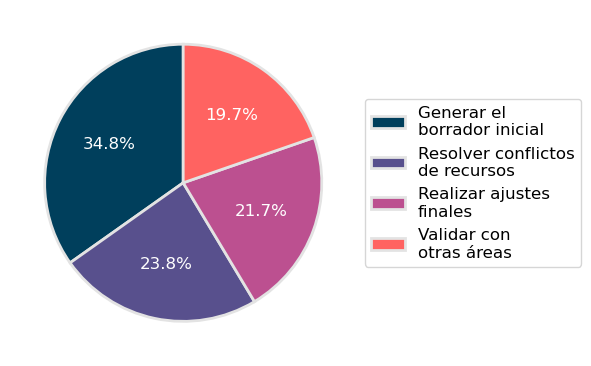
\includegraphics[scale=0.6]{imgs/pie_chart.png}
    \captionsetup{justification=centering} % Para centrar el texto
    \caption{Distribución del tiempo de programación \\ 
    \scriptsize \textbf{Fuente}: Elaboración propia en base a encuesta}
    \label{fig:pie_chart}
\end{figure}
\vfill
\begin{itemize}
    \item Herramientas automatizadas podrían optimizar la generación del cronograma.
    \item Crear el borrador inicial y manejar cambios de último minuto son las necesidades más urgentes.
\end{itemize}
\vfill
\end{frame}


% ---------------------------------------------------
% Sección: Definiciones teóricas
% ---------------------------------------------------
\section{Definiciones teóricas}

% --- FRAME 10: Introducción a la sección ---
\begin{frame}{Definiciones Teóricas}
    Se presentan los conceptos fundamentales para comprender el enfoque del proyecto.
\begin{itemize}
    \vfill
        \arrowitem \textbf{RCPSP} (Problema de Programación de Proyectos con Restricciones de Recursos)
        \arrowitem \textbf{CP} (Programación por Restricciones)

\end{itemize}
\vfill
\end{frame}

% --- FRAME 11: RCPSP - Introducción ---
\subsection{Problema de programación de proyectos con restricciones de recursos (RCPSP)}
\begin{frame}{\textit{RCPSP}: Definición e Importancia}
\begin{itemize}
    \item El \textit{\textbf{RCPSP}} es un problema clásico de investigación operativa y gestión de proyectos.
    \vfill
    \item Pertenece a los \textit{Constraint Satisfaction Problems} (CSP) y, más específicamente, a los \textit{Constraint Optimization Problems} (COP).
    \vfill
    % \item \textbf{Objetivo principal}: determinar el calendario óptimo que minimice el \textit{makespan} (o cualquier otro criterio relevante, como costos o utilización de recursos) \cite{artigues2008resource}.
\end{itemize}
\vfill
\end{frame}

% --- FRAME 13: RCPSP - Ejemplo ---
\begin{frame}{Ejemplo de \textit{RCPSP}}
\begin{figure}
    \centering
    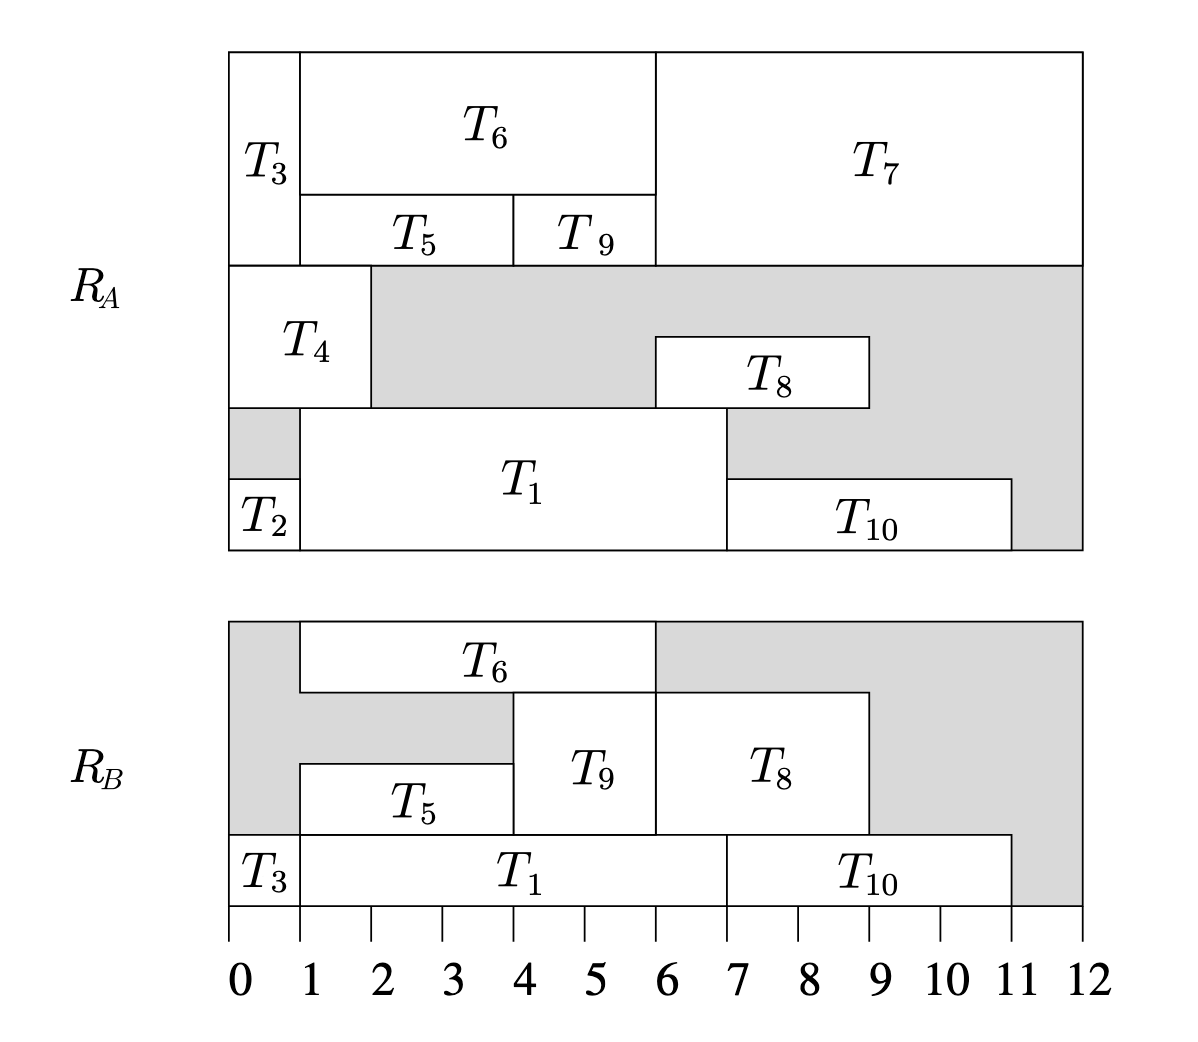
\includegraphics[width=0.4\textwidth]{imgs/rcpsp.png}
    \caption{Ejemplo de un \textit{RCPSP} con 2 recursos y 10 tareas.}
    \label{fig:rcpsp}
\end{figure}
\vfill
\end{frame}

% --- FRAME 12: RCPSP - Características ---
\begin{frame}{Características principales del \textit{RCPSP}}
\begin{itemize}
    \item \textbf{Restricciones de precedencia:} 
    \begin{itemize}
        \arrowitem Algunas actividades no pueden comenzar hasta que otras hayan finalizado.
    \end{itemize}
    \vfill
    \item \textbf{Recursos limitados:}
    \begin{itemize}
        \arrowitem Mano de obra, equipos y materiales con disponibilidad limitada cada periodo.
    \end{itemize}
    \vfill
    \item \textbf{Objetivo de optimización:}
    \begin{itemize}
        \arrowitem Generalmente, minimizar el tiempo total del proyecto (\textit{makespan}).
        \arrowitem También pueden considerarse otros objetivos (costos, carga de recursos, etc.).
    \end{itemize}
\end{itemize}
\vfill
\end{frame}


% --- FRAME 14: RCPSP - Complejidad ---
\begin{frame}{Complejidad del \textit{RCPSP}}
\begin{itemize}
    \item El \textit{RCPSP} es un problema \textit{NP-Hard}, 
    lo que implica un crecimiento exponencial del espacio de soluciones conforme aumenta el número de tareas y recursos.
    \vfill
    \item Para instancias pequeñas, se pueden aplicar métodos exactos; sin embargo, a mayor escala, se requieren enfoques alternativos.
    \vfill
    \item \textbf{Programación por Restricciones (CP)} se presenta como una herramienta eficaz para modelar y resolver el \textit{RCPSP} de manera declarativa.
\end{itemize}
\vfill
\end{frame}

% --- FRAME 15: CP - Introducción ---
\subsection{Algoritmos de programación por restricciones (\textit{CP})}
\begin{frame}{\textit{CP}: Definición e Importancia}
\begin{itemize}
    \item \textit{\textbf{CP}} es una técnica para resolver problemas combinatorios complejos (planificación, programación, optimización).
    \vfill
    \item En este trabajo, \textit{CP} es fundamental para abordar el \textit{RCPSP}, 
    permitiendo modelar restricciones de tiempo y recursos.
\end{itemize}
\vfill
\end{frame}

% --- FRAME 16: CP - Concepto de CSP/COP ---
% \begin{frame}{\textit{CSP} y \textit{COP}}
% \begin{itemize}
%     \item Un \textbf{CSP} (\textit{Constraint Satisfaction Problem}) se define por:
%     \begin{itemize}
%         \arrowitem Un conjunto de variables $V$ con dominios de valores $D$.
%         \arrowitem Un conjunto de restricciones $R$.
%     \end{itemize}
%     \item La solución a un \textbf{CSP} es la asignación de valores a las variables que satisfaga todas las restricciones.
%     \item Un \textbf{COP} (\textit{Constraint Optimization Problem}) incorpora una función objetivo $O$ que se busca optimizar % \cite{rossi2006}.
%     \vfill
%     % \item En un \textit{COP} (\textit{Constraint Optimization Problem}), se incorpora una función objetivo $O$ que se busca optimizar \cite{rossi2006}.
% \end{itemize}
% \vfill
% \end{frame}

% --- FRAME 17: CP - Esquema General ---
\begin{frame}{Esquema de Programación por Restricciones}
\begin{figure}
    \centering
    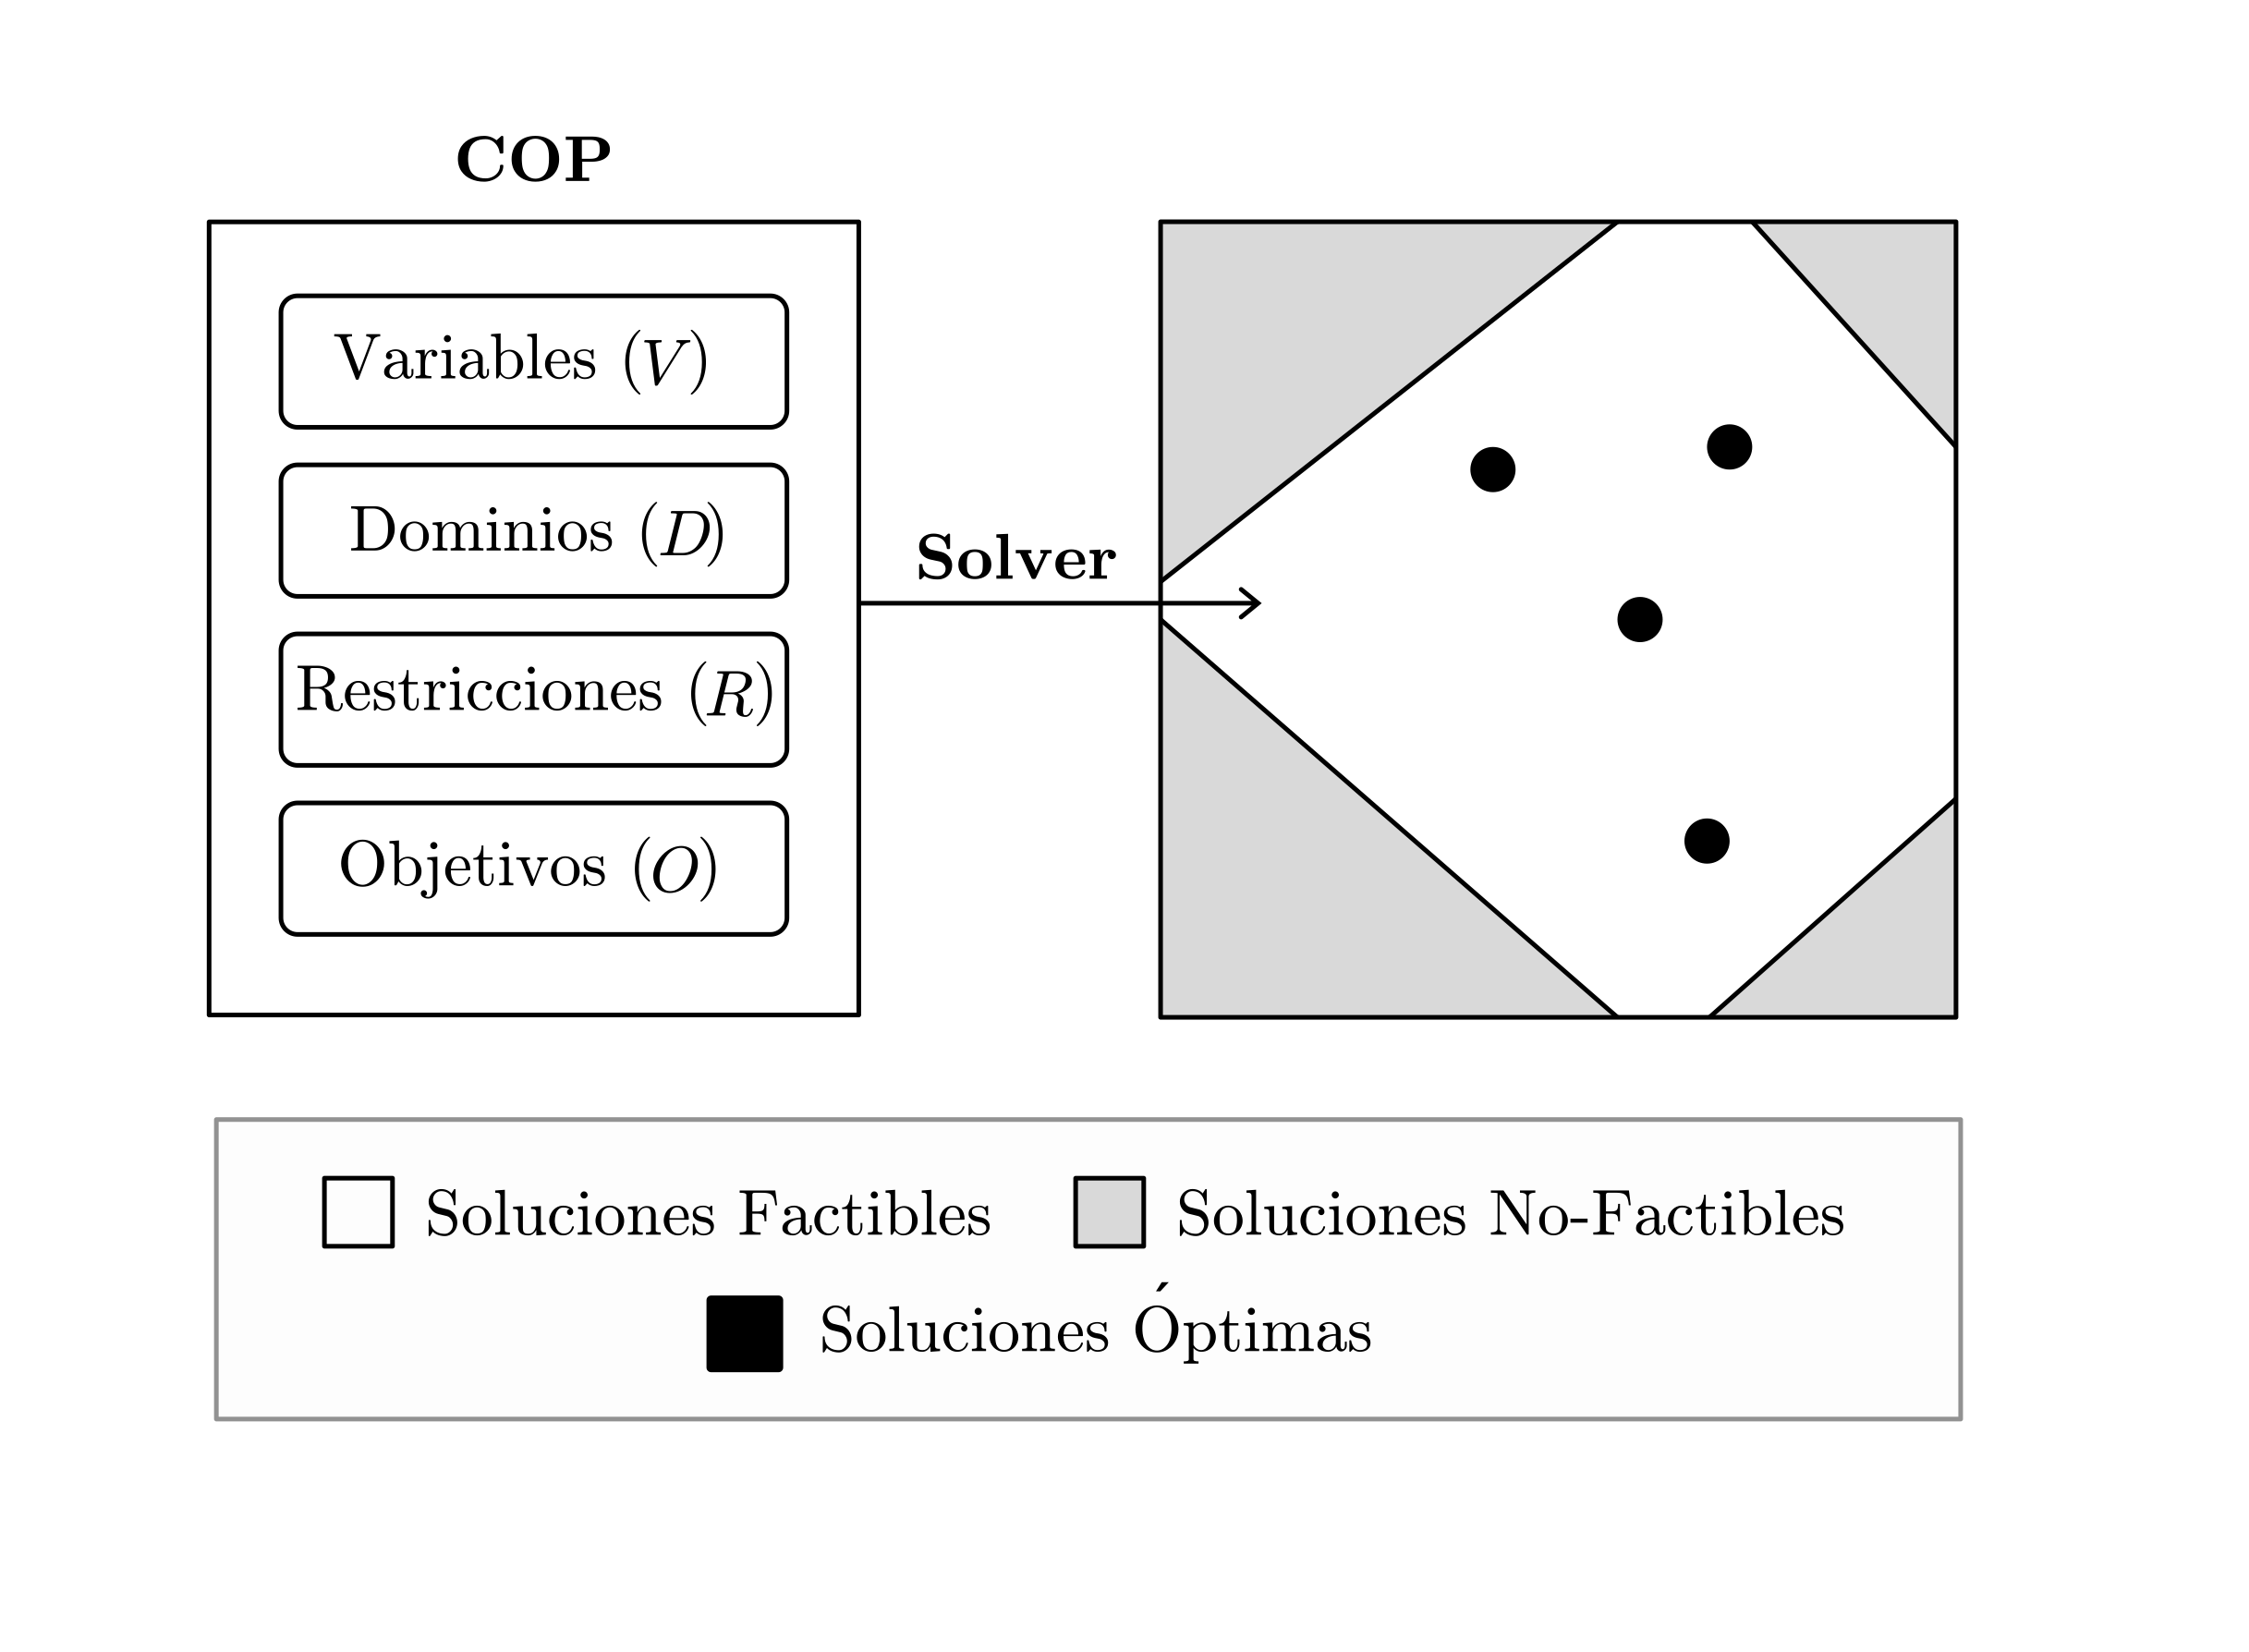
\includegraphics[width=0.52\textwidth]{imgs/constraint_programming.png}
    \caption{Esquema de Programación con Restricciones.}
    \label{fig:constraint_programming}
\end{figure}
\vfill
\end{frame}


% -----------------------------------------------------
% Subsection: Generalización del problema como RCPSP
% -----------------------------------------------------
\section{Aplicación de los conceptos teóricos al problema}
\subsection{Generalización del problema como \textit{RCPSP}}

% --- FRAME 5: Modelado como RCPSP ---
\begin{frame}{Modelado como un \textit{RCPSP}}
\begin{itemize}
    \item \textbf{Objetivo}: Asignar tiempos de inicio a cada tarea, minimizando el \textit{makespan} y 
    la cantidad de tareas no programadas.
    \vfill
    \item Restricciones de:
    \begin{itemize}
        \arrowitem Capacidad de recursos.
        \arrowitem Ventanas de tiempo y precedencia.
        \arrowitem Intervalos prohibidos.
    \end{itemize}
\end{itemize}
\vfill
\end{frame}

% --- FRAME 6: Parámetros del modelo ---
\subsubsection{Parámetros del modelo}
\begin{frame}{Parámetros del modelo}
\begin{itemize}
    \item \textbf{Tareas} \( T = \{T_0, T_1, \dots, T_n\} \):
    \begin{itemize}
        \arrowitem Duración \( C(T_i) \).
        \arrowitem Recursos requeridos \( D(T_i) \) y cantidad \( q_i \).
        \arrowitem Criticidad \( \text{Impact}_i \).
        \arrowitem Ventana de tiempo \( W(T_i) = [\text{early}_i, \text{late}_i] \).
    \end{itemize}
    \vfill
    \item \textbf{Recursos} \( R = \{R_0, R_1, \dots, R_m\} \):
    \begin{itemize}
        \arrowitem Capacidad \( P(R_j) \).
        \arrowitem Intervalos prohibidos \( I(R_j) \).
    \end{itemize}
    \vfill
    \item \textbf{Grupos de tareas} \( G = \{G_0, G_1, \dots\} \):
    \begin{itemize}
        \arrowitem Conjunto de tareas con restricciones de precedencia internas.
    \end{itemize}
\end{itemize}
\vfill
\end{frame}

% --- FRAME 7: Variables de decisión ---
\subsubsection{Variables de decisión}
\begin{frame}{Variables de decisión}
\begin{itemize}
    \item \( x_i \in \{0, 1\} \): Indica si la tarea \( T_i \) es \textbf{programada}.
    \item \( S_i \in \mathbb{N} \): Momento de \textbf{inicio} de la tarea \( T_i \).
    % \item \( E_i = S_i + C(T_i) \): Momento de \textbf{finalización} de la tarea \( T_i \).
    % \item \( \text{Intervalo}(T_i) = [S_i, E_i) \): Intervalo de ejecución.
    % \item \( y_k \in \{0, 1\} \): Indica si el \textbf{grupo de tareas} \( G_k \) se programa.
\end{itemize}
\vfill
\end{frame}

% --- FRAME 8: Restricciones (parte 1) ---
\subsubsection{Restricciones}
\begin{frame}{Restricciones (I)}
\begin{enumerate}
    \item \textbf{Ventanas de tiempo}:
    \[
      x_i = 1 \implies \text{early}_i \leq S_i \leq \text{late}_i - C(T_i)
    \]
    \vfill
    \item \textbf{Capacidad de recursos}:
    \[
      \sum_{\substack{T_i \in T \\ R_j \in D(T_i)}} q_i \cdot \delta_{ij}(t) \leq P(R_j), 
      \quad \forall t \in \text{Horizonte}
    \]
    donde \( \delta_{ij}(t) = 1 \) si \( t \in [S_i, E_i) \) y \( x_i = 1 \), en caso contrario \( \delta_{ij}(t) = 0 \).
\end{enumerate}
\vfill
\end{frame}

% --- FRAME 9: Restricciones (parte 2) ---
\begin{frame}{Restricciones (II)}
\begin{enumerate}
  \setcounter{enumi}{2} % Para continuar la enumeración
    \item \textbf{Intervalos prohibidos}:
    \[
      x_i = 1 \implies \forall R_j \in D(T_i), \forall [a_k, b_k) \in I(R_j):
      \quad [S_i, E_i) \cap [a_k, b_k) = \emptyset
    \]
    \vfill
    \item \textbf{Restricciones de precedencia en grupos}:
    \[
      y_k = 1 \implies \forall (T_i, T_{i+1}) \in G_k: \ S_{i+1} \geq E_i 
      \quad \text{y} \quad \forall T_i \in G_k: x_i = y_k
    \]
    \vfill
    % \item \textbf{Consistencia de variables}:
    % \[
    %   x_i = 0 \implies S_i = 0, \quad E_i = 0
    % \]
\end{enumerate}
\vfill
\end{frame}

% --- FRAME 10: Función objetivo ---
\subsubsection{Objetivo}
\begin{frame}{Función objetivo}
\begin{itemize}
  \item Se desea minimizar \(\textit{makespan}\) y penalizar la no programación de tareas.
  \vfill
  \item Definimos un \textbf{peso} para cada tarea basado en su criticidad:
  \[
  w_i = (\text{Impact}_{\text{max}} + 1 - \text{Impact}_i)^3
  \]
  donde \(\text{Impact}_{\text{max}} = 3\).
  \vfill
  \item \textbf{Función objetivo}:
  \[
  \min Z = \alpha \cdot \text{makespan} 
           + \beta \cdot \sum_{i=0}^{n} w_i \cdot (1 - x_i)
  \]
  \begin{itemize}
      \arrowitem \(\alpha\): Peso asociado al \textit{makespan}.
      \arrowitem \(\beta\): Peso asociado a la no-programación de tareas (según criticidad).
  \end{itemize}
\end{itemize}
\vfill
\end{frame}

% --- FRAME 11: Detalle de la función objetivo ---
\subsection{Detalle de la función objetivo}
\begin{frame}{Detalle de la función objetivo}
    \[
        \min Z = \alpha \cdot \text{makespan} 
                 + \beta \cdot \sum_{i=0}^{n} w_i \cdot (1 - x_i)
        \]
      
\begin{enumerate}
  \item \textbf{Componente Makespan} (\(\alpha \cdot \text{makespan}\)):
  \begin{itemize}
    \arrowitem Minimiza la extensión global del horizonte temporal.
    \arrowitem Promueve la eficiencia en el uso de recursos.
  \end{itemize}
  \vfill
  \item \textbf{Componente Penalización} (\(\beta \cdot \sum w_i (1 - x_i)\)):
  \begin{itemize}
    \arrowitem Permite que ciertas tareas no se programen, pero \textbf{penaliza} fuertemente la no-programación de tareas críticas.
    \arrowitem Evita que el modelo sea infactible si hay incompatibilidades extremas.
  \end{itemize}
\end{enumerate}
\vfill
\end{frame}


% % --- FRAME 12: Balance de objetivos ---
% \begin{frame}{Balance de objetivos}
% \begin{itemize}
%     \item \(\alpha\) y \(\beta\) controlan la preferencia entre un \textit{makespan} menor y la programación de tareas críticas.
%     \vfill
%     \item \(\alpha \gg \beta\): Favorece un \textit{makespan} corto aunque implique no programar algunas tareas.
%     \vfill
%     \item \(\beta \gg \alpha\): Preferencia por programar tantas tareas como sea posible (especialmente las críticas), aun si aumenta el \textit{makespan}.
%     \vfill
%     \item Este balance permite al modelo adaptarse a distintas políticas operativas.
% \end{itemize}
% \vfill
% \end{frame}


% -------------------------------------------------------
% Sección: Aplicación de los conceptos teóricos al problema
% -------------------------------------------------------
\section{Requisitos de la solución}

\subsection{Datos necesarios para el proceso de programación}

% --- FRAME 2: Datos de entrada ---
\begin{frame}{Datos necesarios para la programación}
\begin{itemize}
  \item El \textit{input} principal proviene del proceso de \textbf{planificación}, que define:
  \begin{itemize}
      \arrowitem Ventana de fechas.
      \arrowitem Duración y criticidad de cada tarea.
      \arrowitem Recursos requeridos (cuadrillas, equipo auxiliares).
  \end{itemize}
  \vfill
  \item También se incorporan datos desde el sistema \textit{ERP}:
  \begin{itemize}
      \arrowitem Turnos de las cuadrillas.
      \arrowitem Disponibilidad de equipos auxiliares.
  \end{itemize}
  \vfill
%   \item Disponibilidad de \textbf{materiales y repuestos} no se considera debido a la falta de sistematización en el \textit{ERP}.
\end{itemize}
\vfill
\end{frame}

% --- FRAME 3: Tabla de ejemplo de Tarea ---
\begin{frame}[fragile]{Ejemplo de Tarea y sus atributos}
\vspace{-2ex}
\scriptsize
\begin{table}[htbp]
    \centering
    \captionsetup{justification=centering}
    \vspace{0.3cm}
    \begin{tabular}{p{4cm} p{5.5cm}}
        \toprule
        \textbf{Atributo} & \textbf{Descripción} \\
        \midrule
        \textbf{ID Orden de Trabajo} & 4000001 \\
        \textbf{ID Tarea} & 001 \\
        \textbf{Descripción OT} & Cambio de suspensión trasera lado izquierdo \\
        \textbf{Descripción Tarea} & Retiro de suspensión trasera \\
        \textbf{Fecha Inicio Extrema} & 2024-11-29 \\
        \textbf{Fecha Requerida} & 2024-12-30 \\
        \textbf{Cuadrilla} & BM001 \\
        \textbf{Equipo Auxiliar} & Alza Hombres Telescópico \\
        \textbf{Duración (horas)} & 6 \\
        \textbf{Criticidad} & 2 \\
        \textbf{Cantidad de Trabajadores} & 4 \\
        \bottomrule
    \end{tabular}
    \caption{Ejemplo de Tarea y sus atributos }%\cite{tabla:fuente}.}
    \label{table:task}
\end{table}
\vfill
\end{frame}


% -----------------------------------------------------
% Subsection: Consideraciones al programar
% -----------------------------------------------------
\subsection{Consideraciones al programar}

% --- FRAME 4: Consideraciones al programar ---
\begin{frame}{Consideraciones al programar}
\begin{itemize}
    % \item Cada \textbf{tarea} incluye:
    % \begin{itemize}
    %   \arrowitem Fecha de inicio extrema y requerida.
    %   \arrowitem Duración y criticidad.
    %   \arrowitem Recursos requeridos (cuadrillas, equipos).
    % \end{itemize}
    % \vfill
    \item \textbf{Restricciones de precedencia} dentro de la orden de trabajo (OT).
    \vfill
    \item \textbf{Cuadrillas}:
    \begin{itemize}
      \arrowitem Tienen esquemas de turnos (disponibilidad limitada).
      \arrowitem Cuentan con una capacidad (número de trabajadores) que determina cuántas tareas en paralelo pueden atender.
    \end{itemize}
    \vfill
    \item \textbf{Equipos auxiliares} son recursos unitarios (no se comparten en simultáneo).
    \vfill
    \item \textbf{Cronograma base}: Se parte de cronogramas anteriores para ajustarlos e incorporar nuevas tareas.
    \vfill
    % \item Si se programa una tarea de una \textbf{OT}, se programan todas las tareas de dicha OT.
\end{itemize}
\vfill
\end{frame}

\begin{frame}{Requisitos de la solución}
    \begin{itemize}
        \item \textbf{Eficiencia}: Procesamiento rápido y generación de cronogramas en tiempo real.
        \vfill
        \item \textbf{Escalabilidad}: Capacidad de manejar grandes volúmenes de tareas y recursos.
        \vfill
        \item \textbf{Flexibilidad}: Adaptación a cambios de último minuto y restricciones dinámicas. La solución debe ser capaz de partir de un cronograma base y ajustarlo, minimizando la cantidad de cambios.
        \vfill
        \item \textbf{Usabilidad}: Interfaz amigable y fácil de usar para el personal de programación. 
    \end{itemize}
    \vfill
    \end{frame}
    


% ---------------------------------------------------
% Sección: Diseño de la solución
% ---------------------------------------------------
\section{Diseño de la solución}

% --- FRAME 2: Visión General del Flujo de Trabajo ---
\begin{frame}{Flujo de Trabajo de la Solución}
\begin{figure}
    \centering
    
\includegraphics[width=0.9\textwidth]{imgs/solution.png}
    \caption{Flujo de Trabajo de la Solución.}
    \label{fig:solution}
\end{figure}
\begin{columns}[t] % [t] alinea las columnas en la parte superior
    \begin{column}{0.5\textwidth}
        \begin{enumerate}
            \item Pre-Procesamiento
            \item Segmentación en Subconjuntos
        \end{enumerate}
    \end{column}
    \begin{column}{0.5\textwidth}
        \begin{enumerate} % Retoma la numeración
            \setcounter{enumi}{2}
            \item \textit{Solver}
            \item Post-Procesamiento
        \end{enumerate}
    \end{column}
\end{columns}

\vfill
\end{frame}

% ---------------------------------------------------
% Subsection: Pre-procesamiento
% ---------------------------------------------------
\subsection{Pre-procesamiento}

% --- FRAME 3: Pre-Procesamiento ---
\begin{frame}{1. Pre-Procesamiento}
\begin{itemize}
    \item \textbf{Objetivo}: Limpiar y preparar la información procedente de las fuentes de datos (\textit{ERP}, \textit{Microsoft Project}, u otros formatos).
    \vfill
    \item Operaciones clave:
    \begin{itemize}
        \arrowitem \textbf{Corrección de discrepancias}: Ajuste automático de errores (ej. fechas incoherentes).
        \arrowitem \textbf{Cuantización de ventanas horarias}: Expresar duraciones en intervalos de 15 minutos para optimizar el modelado.
        % \arrowitem \textbf{Restringir horarios fijos}: Configurar intervalos obligatorios para ciertas tareas.
        \arrowitem \textbf{Estandarización en JSON}: Consolidación de datos (duraciones, recursos, dependencias) en un formato coherente.
    \end{itemize}
\end{itemize}
\vfill
\end{frame}

% ---------------------------------------------------
% Subsection: Segmentación en Subconjuntos
% ---------------------------------------------------
\subsection{Segmentación en Subconjuntos}


% --- FRAME 5: Ejemplo de Segmentación ---
\begin{frame}{2. Segmentación en Subconjuntos}
    \begin{figure}
        \centering
        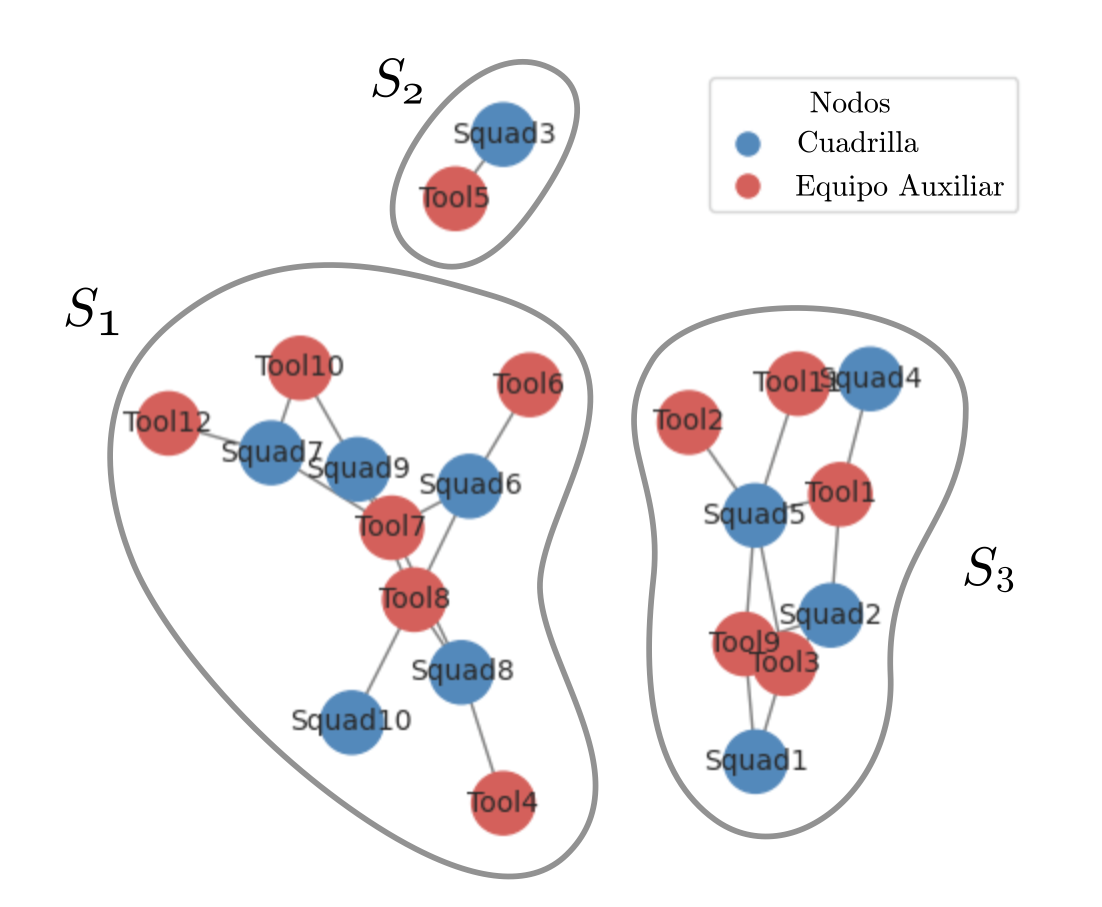
\includegraphics[width=0.45\textwidth]{imgs/segmentacion.png}
        \caption{Ejemplo de segmentación a través de componentes conexos.}
        \label{fig:segmentacion}
    \end{figure}
    \vfill
\end{frame}

% --- FRAME 4: Segmentación en Subconjuntos ---
\begin{frame}{Metodología de Segmentación}
\begin{itemize}
    \item \textbf{Objetivo}: Reducir la complejidad del problema al dividirlo en grupos más pequeños.
    \vfill
    \item \textbf{Método}:
    \begin{enumerate}
        \item \textbf{Construcción del grafo}: Cuadrillas y equipos como nodos; existe arista si hay tareas que usan ambos recursos de forma simultánea.
        \item \textbf{Componentes conexos}: Identificación de grupos interrelacionados que se tratarán como un subconjunto.
        \item \textbf{Formación de subconjuntos}: Cada componente conexo se resuelve de manera independiente en el \textit{solver}.
    \end{enumerate}
\end{itemize}
\vfill
\end{frame}

% ---------------------------------------------------
% Subsection: Solver
% ---------------------------------------------------
\subsection{\textit{Solver}}

% --- FRAME 6: Solver - Diccionarios de entrada ---
\begin{frame}{3. \textit{Solver}: Construcción de \textit{input}}
\begin{itemize}
    \item Uso de \textit{OR-Tools} (CP-SAT solver) para modelar y resolver el \textit{RCPSP}.
    \vfill
    \item \textbf{add\_hint}: Permite incorporar soluciones anteriores o ajustes del usuario como punto de partida.
    \item Cada subconjunto se resuelve de forma independiente, pudiendo ejecutarse en paralelo (\textit{joblib}, hilos, múltiples núcleos).
    \vfill
    \item \textbf{Ventajas de la paralelización}:
    \begin{itemize}
        \arrowitem Aprovecha mejor los recursos de hardware.
        \arrowitem Reduce el tiempo total de ejecución.
    \end{itemize}
    \vfill
    \item Se obtiene una solución parcial por cada subconjunto, que luego se unifica.
\end{itemize}
\vfill
\end{frame}


% ---------------------------------------------------
% Subsection: Post-procesamiento
% ---------------------------------------------------
\subsection{Post-procesamiento}

% --- FRAME 8: Post-Procesamiento ---
\begin{frame}{4. Post-Procesamiento}
\begin{itemize}
    \item \textbf{Objetivo}: Consolidar y preparar la salida del \textit{solver} para su integración y análisis final.
    \vfill
    \item Salidas principales:
    \begin{itemize}
        \arrowitem \textbf{Archivos XML para MS Project}: Permite incorporar el cronograma a entornos de gestión existentes.
        \arrowitem \textbf{Archivo XLSX (Gantt)}: Visualización rápida de la programación en hojas de cálculo.
        \arrowitem \textbf{Integraciones con APIs}: Conexión automática con sistemas \textit{ERP} o herramientas empresariales.
    \end{itemize}
\end{itemize}
\vfill
\end{frame}




% -----------------------------------------------
% Sección: Resultados y Análisis
% -----------------------------------------------
\section{Resultados y análisis}

% --- FRAME 1: Introducción a la sección ---
% \begin{frame}{Resultados y análisis}
% \begin{itemize}
%     \item Se presentan los resultados clave del modelo de optimización.
%     \vfill
%     \item Se analiza:
%     \begin{itemize}
%         \arrowitem El conjunto de datos utilizado.
%         \arrowitem El ajuste de parámetros en la función objetivo.
%         \arrowitem El impacto de la segmentación en subconjuntos.
%     \end{itemize}
%     \vfill
%     \item Beneficios operativos proyectados para el equipo de programación.
% \end{itemize}
% \vfill
% \end{frame}

% -----------------------------------------------
% Subsection: Descripción del conjunto de datos
% -----------------------------------------------
\subsection{Descripción del conjunto de datos}

% --- FRAME 2: Conjunto de Datos (Tabla) ---
\begin{frame}{Conjunto de datos: Características generales}
\begin{itemize}
    \item Datos reales provistos por la empresa colaboradora.
    \item Período de planificación: Del 17 de julio al 3 de agosto de 2023.
    \vfill
\end{itemize}

\scriptsize
\begin{table}[htbp]
    \centering
    \begin{tabular}{lc}
        \toprule
        \textbf{Atributo} & \textbf{Valor} \\
        \midrule
        Número total de tareas & 4.898 \\
        Número de órdenes de trabajo (OT) & 1.055 \\
        Fecha mínima & 2023/07/17 \\
        Fecha máxima & 2023/08/03 \\
        Duración promedio (horas) & 1,92 \\
        Número de cuadrillas & 31 \\
        Número de equipos auxiliares & 16 \\
        \bottomrule
    \end{tabular}
    \caption{Resumen de las características del conjunto de datos.}
    \label{tab:dataset_summary}
\end{table}
\vfill
\end{frame}

% --- FRAME 3: Criticidad de las Tareas (Figura) ---
% \begin{frame}{Distribución de tareas según criticidad}
% \begin{columns}
%     \begin{column}{0.5\textwidth}
%         \begin{itemize}
%             \item \textbf{Criticidad 1 (Alta)}: 666 tareas (13,6\%)
%             \item \textbf{Criticidad 2 (Media)}: 2.403 tareas (49,1\%)
%             \item \textbf{Criticidad 3 (Baja)}: 1.829 tareas (37,3\%)
%         \end{itemize}
%         \vfill
%         \textbf{Recursos}:
%         \begin{itemize}
%             \arrowitem 31 cuadrillas (distintos turnos y capacidades).
%             \arrowitem 16 equipos auxiliares (recursos unitarios).
%         \end{itemize}
%     \end{column}
%     \begin{column}{0.45\textwidth}
%         \begin{figure}
%             \centering
%             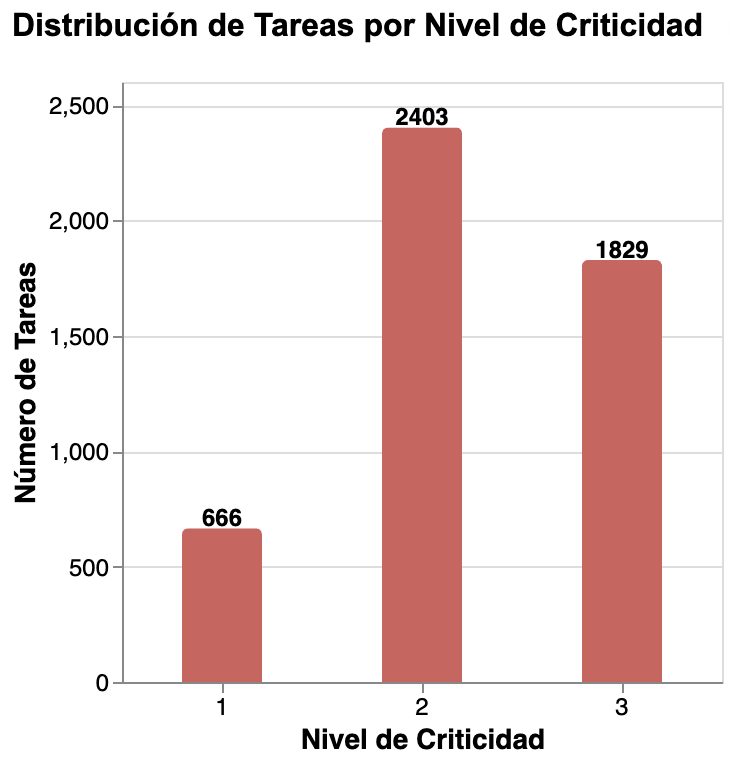
\includegraphics[width=0.8\textwidth]{imgs/barras_impacto.png}
%             \caption{Distribución de tareas según criticidad.}
%             \label{fig:barras_impacto}
%         \end{figure}
%     \end{column}
% \end{columns}
% \vfill
% \end{frame}

% -----------------------------------------------
% Subsection: Ajuste de parámetros
% -----------------------------------------------
\subsection{Ajuste de parámetros para la función objetivo}

% --- FRAME 4: Función objetivo y experimentos ---
\begin{frame}{Resultados para distintos \(\alpha\) y \(\beta\)}
\begin{itemize}
    \item La función objetivo combina:
    \[
    \min Z = \alpha \cdot \text{makespan} 
             + \beta \cdot \sum_{i=0}^{n} w_i \cdot (1 - x_i)
    \]
  
    \begin{itemize}
        \arrowitem \(\alpha\): Peso del \textit{makespan}.
        \arrowitem \(\beta\): Penalización por no programar tareas (enfocada en criticidad).
    \end{itemize}
    \vfill
    \item Múltiples experimentos con distintas combinaciones (\(\alpha, \beta\)) para analizar:
    \begin{itemize}
        \arrowitem Número total de tareas programadas.
        \arrowitem Tareas no programadas por criticidad.
        \arrowitem \textit{Makespan}.
        \arrowitem Tiempo de solución.
    \end{itemize}
\end{itemize}
\vfill
\end{frame}

% --- FRAME 5: Resultados Generales (Tabla) ---
\begin{frame}{Resultados Generales (\(\alpha\)-\(\beta\))}
\begin{table}[htbp]
    \centering
    \footnotesize
    \begin{tabular}{c c c c c c c}
        \toprule
        \textbf{Conf.} & \(\alpha\) & \(\beta\) & 
        \makecell{\textbf{Tareas} \\ \textbf{Prog.}} & 
        \makecell{\textbf{Tareas no} \\ \textbf{Prog.}} & 
        \makecell{\textbf{Tiempo Sol.} \\ \textbf{(s)}} & 
        \textbf{Makespan} \\
        \midrule
        (a) & 1 & 0 & 0 & 4.898 & 3,43 & 0 \\
        (b) & 0 & 1 & 4.854 & 44 & 4,35 & 1.072 \\
        (c) & 1 & 1 & 4.658 & 240 & 8,42 & 492,75 \\
        (d) & 1 & 2 & 4.831 & 67 & 9,95 & 516,25 \\
        \bottomrule
    \end{tabular}
    \caption{Resultados con diferentes configuraciones de \(\alpha\) y \(\beta\).}
    \label{tab:alpha_beta_general}
\end{table}
\vfill
\end{frame}

% --- FRAME 6: Distribución de Tareas no Programadas ---
\begin{frame}{Distribución de Tareas no Programadas por Criticidad}
    \begin{table}[htbp]
        \centering
        \footnotesize
        \begin{tabular}{c c c c c c}
            \toprule
            \textbf{Conf.} & \(\alpha\) & \(\beta\) & 
            \textbf{Criticidad 1} & 
            \textbf{Criticidad 2} & \textbf{Criticidad 3} \\
            \midrule
            (a) & 1 & 0 & 666 & 2.403 & 1.829 \\
            (b) & 0 & 1 & 0   & 8     & 36 \\
            (c) & 1 & 1 & 21  & 59    & 160 \\
            (d) & 1 & 2 & 0   & 12    & 55 \\
            \bottomrule
        \end{tabular}
        \caption{Tareas no programadas, según criticidad, en cada configuración.}
        \label{tab:alpha_beta_impact}
    \end{table}
    \vfill
\end{frame}

\begin{frame}{Eleccion de \(\alpha\) y \(\beta\)}
    \textbf{Conclusiones}:
    \begin{itemize}
        \arrowitem \((a)\): Minimiza \textit{makespan}, pero no programa ninguna tarea.
        \arrowitem \((b)\): Maximiza tareas programadas (incluye todas las críticas), pero \textit{makespan} muy alto.
        \arrowitem \((c)\): Menor \textit{makespan} pero muchas tareas críticas no programadas.
        \arrowitem \((d)\): Equilibrio entre ambas metas: 4.831 tareas programadas (0 tareas críticas no programadas) y 516,25 h de \textit{makespan}.
    \end{itemize}
    \vfill
    \end{frame}
% -----------------------------------------------
% Subsection: Resultados segmentación
% -----------------------------------------------
\subsection{Resultados de la segmentación en subconjuntos}

% --- FRAME 7: Segmentación en Subconjuntos (Resumen) ---
\begin{frame}{Optimización mediante Segmentación en Subconjuntos}
    \begin{itemize}
        \item El objetivo es reducir la complejidad del problema y \textbf{acelerar el tiempo de solución}.
        \item A modo de \textit{benchmark}, el tiempo de solucion sin segmentación fue de \textbf{9,95 s}.
        \item Se dividió el total de 4.898 tareas en \textbf{14 subconjuntos}.
        \item Reducción de complejidad y paralelización del \textit{solver}.
    \end{itemize}
    \vfill
\end{frame}

\begin{frame}{Segmentación en Subconjuntos}
\begin{table}[htbp]
    \centering
    \footnotesize
    \begin{tabular}{cccc}
        \toprule
        \textbf{Subc.} & \textbf{Tareas} & \(\%\) \textbf{del total} & \textbf{Tiempo Sol. (s)} \\
        \midrule
        S1 & 2.598 & 53\% & 4,34 \\
        S2 & 674   & 14\% & 0,65 \\
        S3 & 319   & 7\%  & 0,43 \\
        S4 & 254   & 5\%  & 0,12 \\
        S5 & 198   & 4\%  & 0,01 \\
        S6 & 136   & 3\%  & 0,01 \\
        S7 & 122   & 2\%  & 0,00 \\
        S8 & 110   & 2\%  & 0,01 \\
        S9 & 98    & 2\%  & 0,00 \\
        S10 & 87   & 2\%  & 0,00 \\
        S11 & 84   & 2\%  & 0,01 \\
        S12 & 78   & 2\%  & 0,00 \\
        S13 & 72   & 1\%  & 0,00 \\
        S14 & 68   & 1\%  & 0,00 \\
        \bottomrule
    \end{tabular}
    \caption{Resultados de la segmentación en subconjuntos.}
    \label{tab:subsets_results}
\end{table}
\vfill
\end{frame}


% --- FRAME 8: Tiempo total y Conclusiones Segmentación ---
\begin{frame}{Tiempo total y conclusiones de la segmentación}
\begin{itemize}
    \item El tiempo de solución total equivale al máximo de todos los subconjuntos: \(\sim 4,34\) s.
    \vfill
    \item Paralelización:
    \begin{itemize}
        \arrowitem Cada subconjunto se procesa en hilos o núcleos distintos.
        \arrowitem Aprovechamiento óptimo del hardware disponible.
    \end{itemize}
    \vfill
    \item Subconjuntos más pequeños (\(<5\%\)) se resuelven casi instantáneamente.
    \vfill
    \item \textbf{Conclusión}: El enfoque modular y paralelo disminuye significativamente el tiempo total de ejecución sin sacrificar la calidad del cronograma.
\end{itemize}
\vfill
\end{frame}

% ---------------------------------------------------
% Sección: Conclusiones y pasos a seguir
% ---------------------------------------------------
\section{Conclusiones y pasos a seguir}

% --- FRAME 1: Conclusiones generales ---
\begin{frame}{Conclusiones Generales}
\begin{itemize}
    \item Se alcanzaron los objetivos propuestos, logrando una \textbf{solución eficiente} para
    la programación automatizada de mantenimiento.
    \vfill
    \item En un conjunto de 4.898 tareas:
    \begin{itemize}
        \arrowitem 98,6\% de tareas programadas (solo 67 no programadas).
        \arrowitem \textbf{Todas} las tareas de criticidad 1 fueron incluidas.
        \arrowitem \textit{Makespan}: 21,5 días.
    \end{itemize}
    \vfill
    \item \textbf{Tiempo total de cálculo:} 6,12 segundos (incluye pre-procesamiento, segmentación,
    resolución y post-procesamiento).
    \vfill
\end{itemize}
\vfill
\end{frame}

% --- FRAME 2: Ejemplo de Gantt en MS Project ---
\begin{frame}{Cronograma Resultante en MS Project}
\centering
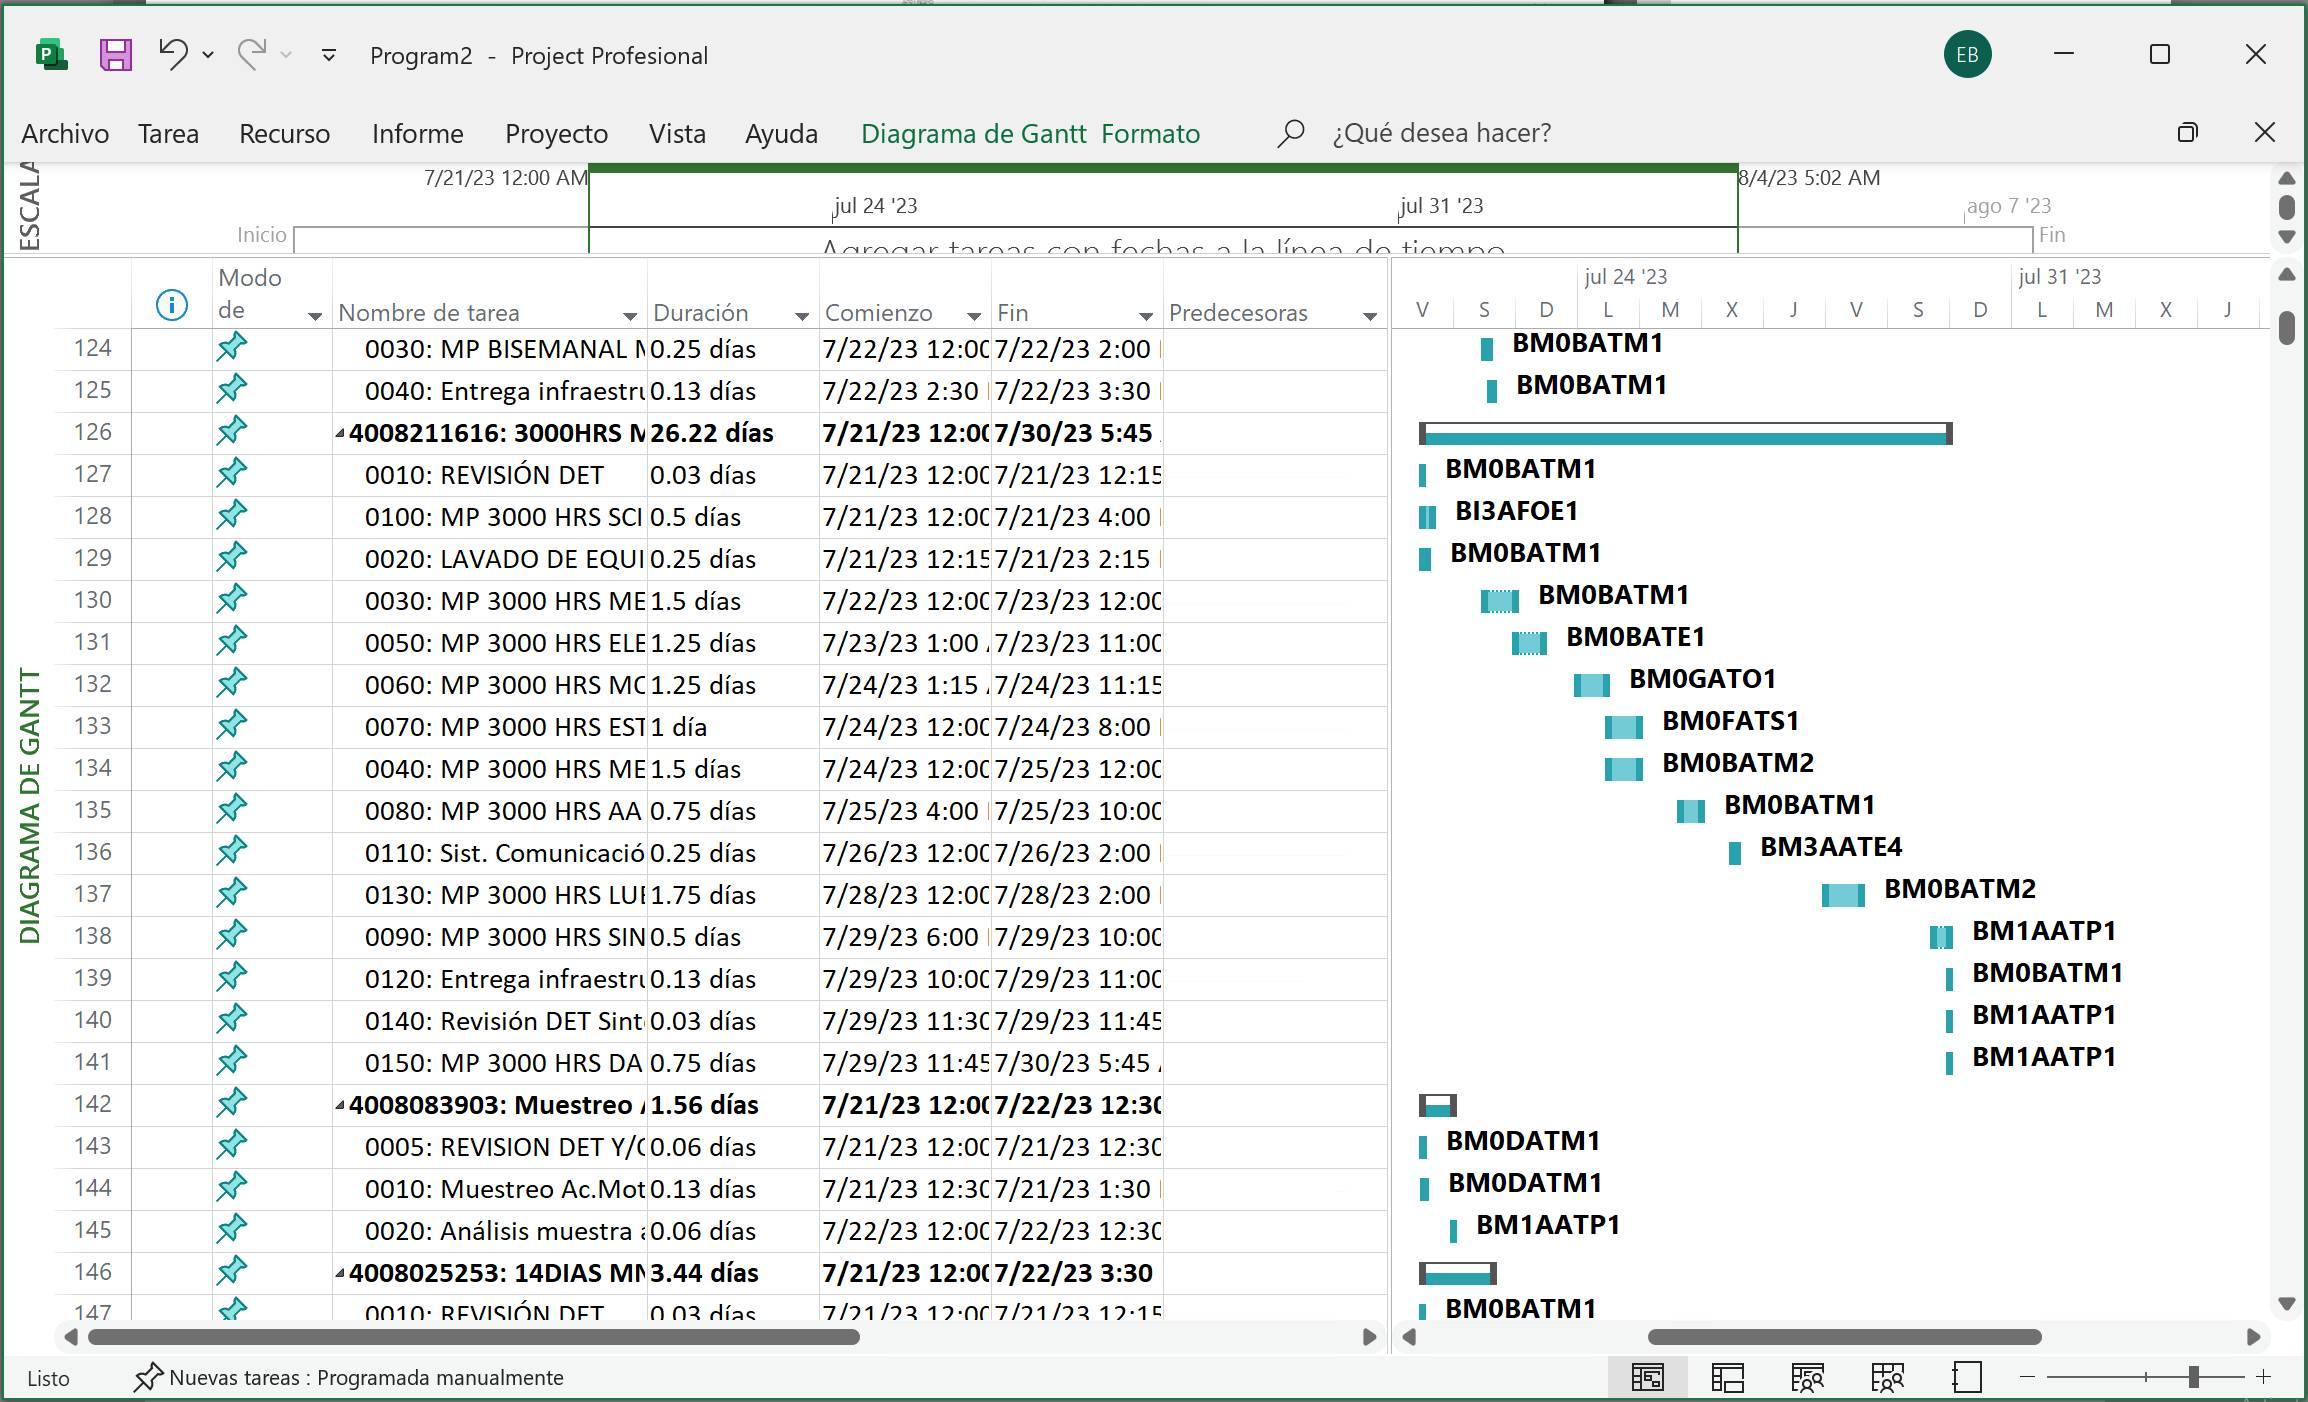
\includegraphics[scale=0.22]{imgs/gantt-project.jpg}
\captionof{figure}{Captura de Cronograma Resultante en \textit{MS Project}}% \cite{refMSProject}.}
\label{fig:gantt-project}
\vfill
\end{frame}

% --- FRAME 3: Impacto sobre proceso de programación ---
\subsection{Impacto sobre el proceso de programación}
\begin{frame}{Impacto estimado sobre el proceso de programación}
\begin{itemize}
    \item La herramienta automatiza completamente la generación del \textbf{borrador inicial}, eliminando la necesidad de hacerlo manualmente.
    \vfill
    \item Permite realizar \textbf{ajustes finos} sobre el borrador inicial, como:
    \begin{itemize}
        \arrowitem Fijar tareas en horarios específicos.
        \arrowitem Modificar disponibilidad de recursos.
        \arrowitem Incorporar tareas de último minuto.
    \end{itemize}
    Durante estos ajustes, el programa adapta automáticamente las tareas relacionadas para garantizar un cronograma viable, reduciendo a la mitad el tiempo necesario para este proceso.
    \vfill
    \item Se estima por lo tanto una reducción total del \(\sim57,6\%\) en el tiempo necesario para la creación del cronograma final.
\end{itemize}
\vfill
\end{frame}

% --- FRAME 4: Limitaciones y consideraciones ---
\subsection{Limitaciones y consideraciones}
\begin{frame}{Limitaciones y consideraciones}
\begin{itemize}
    \item \textbf{Disponibilidad de materiales y repuestos}:
    \begin{itemize}
        \arrowitem Principal error detectado.
        \arrowitem No sistematizado en el \textit{ERP}, por lo que no fue incluido en la solución.
    \end{itemize}
    \vfill
    \item Para integrar este aspecto se requiere:
    \begin{itemize}
        \arrowitem Paso previo de \textbf{gobernanza de datos}.
        \arrowitem Procesos robustos de manejo en bodega.
        \arrowitem Sistematización de información de repuestos.
    \end{itemize}
    \vfill
    \item Sin estos pasos, la herramienta no reduce errores por falta de materiales,
    requiriendo colaboración y compromiso de otras áreas.
\end{itemize}
\vfill
\end{frame}

% --- FRAME 5: Pasos a seguir ---
\subsection{Pasos a seguir}
\begin{frame}{Pasos a seguir: Módulos de Desarrollo de la Solución}
\begin{figure}
    \centering
    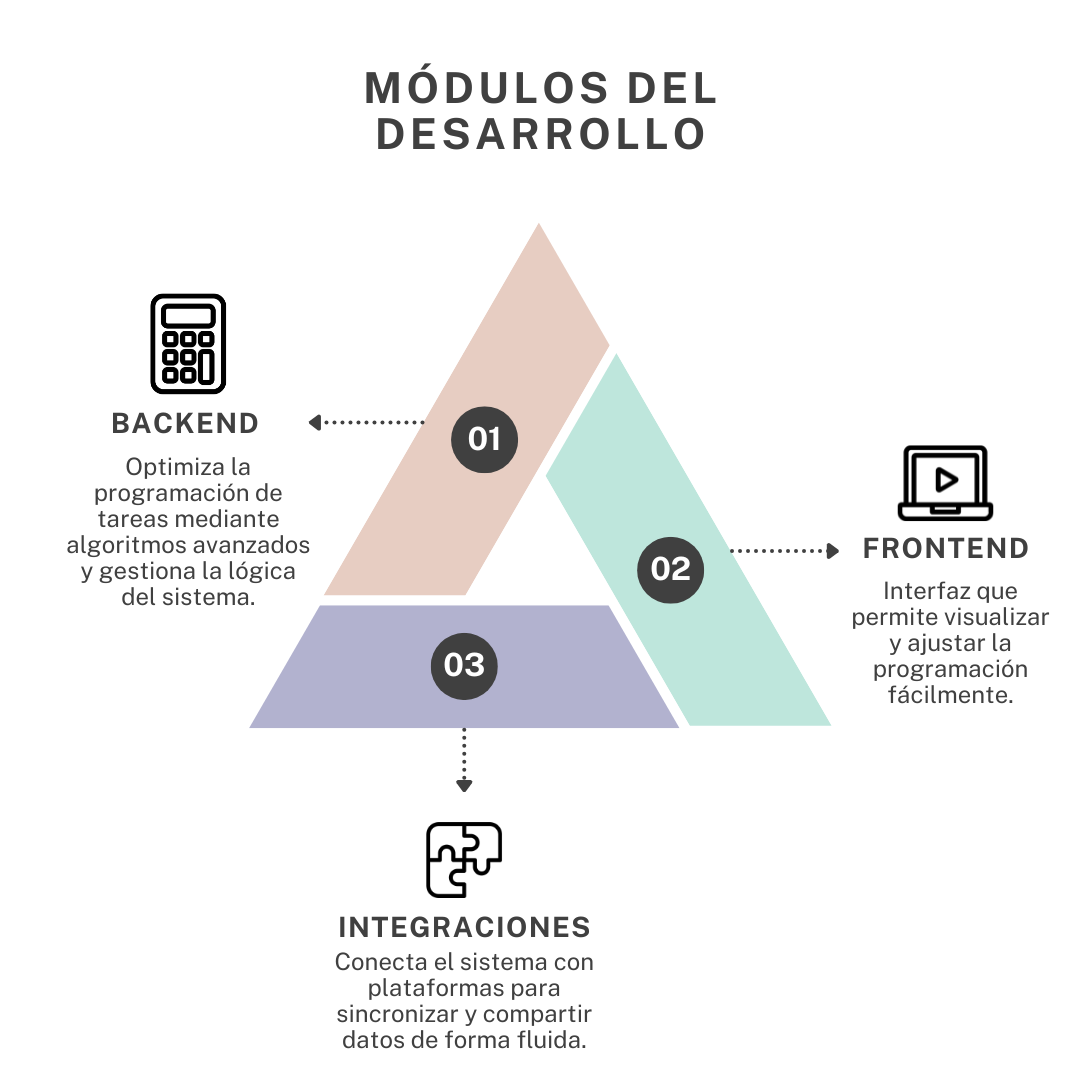
\includegraphics[scale=0.2]{imgs/ModulosDesarrollo.png}
    \caption{Propuesta de Módulos de Desarrollo de Solución.}
    \label{fig:modulos-desarrollo}
\end{figure}
\vfill
\end{frame}

\begin{frame}{Estructura de la Solución}
    \begin{itemize}
        \item \textbf{Backend:} 
        \begin{itemize}
            \arrowitem Coordina y paraleliza la ejecución del \textit{solver}.
            \arrowitem Centraliza los datos y gestiona la comunicación con la base de datos.
            \arrowitem Garantiza la escalabilidad y estabilidad del sistema.
        \end{itemize}
        \vfill
        \item \textbf{Frontend:}
        \begin{itemize}
            \arrowitem Ofrece una interfaz clara e intuitiva para los programadores.
            \arrowitem Facilita la carga de datos, la edición de cronogramas y la revisión de resultados.
            \arrowitem Permite visualizar la información de forma amigable y comprensible.
        \end{itemize}
        \vfill
        \item \textbf{Integración con la plataforma de la empresa:}
        \begin{itemize}
            \arrowitem Conecta la solución con sistemas existentes (p.ej. ERP).
            \arrowitem Asegura la importación y exportación de datos de manera automatizada.
            \arrowitem Mantiene la información sincronizada y actualizada en todo momento.
        \end{itemize}
    \end{itemize}
    \end{frame}

\subsection{Reflexiones finales}
\begin{frame}{Reflexiones finales}
\begin{itemize}
    \item \textbf{Objetivo cumplido}: Se desarrolló una herramienta capaz de automatizar la programación de actividades de mantenimiento con alta eficiencia.
    \vfill
    \item \textbf{Reducción de errores y carga de trabajo}: Se estima que la herramienta permitirá reducir significativamente el tiempo necesario para las tareas de programación además de disminuir errores.
    \vfill
    \item \textbf{Limitaciones}: La falta de sistematización de información sobre materiales y repuestos es una limitación importante que debe ser abordada en futuras etapas.
    \item \textbf{Adopción en la realidad operativa}: Para que la herramienta sea incorporada de manera efectiva,
          se requiere:
    \begin{itemize}
        \item Una \textbf{interfaz intuitiva} y fácil de usar.
        \item \textbf{Integración} confiable con las plataformas de la empresa.
    \end{itemize}
    \vfill
\end{itemize}
\vfill
\end{frame}

% ----Ref Frame--------

\begin{frame}{Bibliography}
\tiny 
\bibliographystyle{apalike}
\bibliography{ref.bib}
\end{frame}


\end{document}
